\documentclass[12pt,a4paper]{article}

\usepackage[utf8]{inputenc}
\usepackage[T1]{fontenc}
\usepackage{graphicx}
\usepackage{hyperref}
\usepackage{geometry}
\usepackage{booktabs}
\usepackage{float}
\usepackage{enumitem}
\usepackage{fancyhdr}
\usepackage{xcolor}
\usepackage{listings}
\usepackage{tikz}
\usepackage{colortbl}
\usepackage{mdframed}
\usepackage{fontawesome5}
\usepackage{setspace}

\geometry{margin=1in, headheight=15pt}
\onehalfspacing

\definecolor{primaryblue}{RGB}{26, 115, 232}
\definecolor{darkblue}{RGB}{13, 71, 161}
\definecolor{lightblue}{RGB}{232, 245, 253}
\definecolor{successgreen}{RGB}{46, 125, 50}
\definecolor{lightgray}{RGB}{248, 249, 250}

\hypersetup{colorlinks=true, linkcolor=darkblue, urlcolor=primaryblue}

\lstset{
    basicstyle=\ttfamily\small,
    breaklines=true,
    frame=single,
    backgroundcolor=\color{lightgray},
    numbers=left,
    numberstyle=\tiny\color{gray},
    keywordstyle=\color{primaryblue}\bfseries,
    rulecolor=\color{gray}
}

\newmdenv[
    linecolor=primaryblue,
    backgroundcolor=lightblue,
    linewidth=2pt,
    topline=false,
    rightline=false,
    bottomline=false,
]{highlightblock}

\newmdenv[
    linecolor=successgreen,
    backgroundcolor=successgreen!10,
    linewidth=2pt,
    topline=false,
    rightline=false,
    bottomline=false,
]{successblock}

\pagestyle{fancy}
\fancyhf{}
\fancyhead[L]{\small\color{gray}Individual Contribution Report}
\fancyhead[R]{\small\color{darkblue}\textbf{Aditya Verma}}
\fancyfoot[C]{\thepage}
\renewcommand{\headrulewidth}{0.5pt}
\renewcommand{\footrulewidth}{0.5pt}

\begin{document}

%========================================
% TITLE PAGE
%========================================
\begin{titlepage}
    \centering
    \vspace*{2cm}
    
    {\Large\color{gray} INDIVIDUAL CONTRIBUTION REPORT\\[0.3cm]}
    
    \rule{0.8\textwidth}{1pt}\\[0.5cm]
    
    {\Huge\bfseries\color{darkblue} Aditya Verma\\[0.5cm]}
    
    \rule{0.8\textwidth}{1pt}\\[1cm]
    
    {\Large\textit{Garbage Classifier for Waste Management}\\[0.3cm]}
    {\large AI-Powered Garbage Segmentation System\\[1.5cm]}
    
    \begin{tikzpicture}
        \node[draw=primaryblue, fill=lightblue, rounded corners=10pt, minimum width=8cm, minimum height=3cm, align=center] {
            \textbf{\large Primary Roles}\\[0.3cm]
            \faIcon{tools} Utility Development\\
            \faIcon{rocket} Deployment Support\\
            \faIcon{presentation} Presentation
        };
    \end{tikzpicture}
    
    \vfill
    
    {\large
    \textbf{BTech (Hons.) CSE - Artificial Intelligence}\\
    5th Semester | Group 09\\[0.5cm]
    University Teaching Department (UTD)\\
    CSVTU, Bhilai\\[0.5cm]
    \textbf{December 2025}
    }
    
\end{titlepage}

\tableofcontents
\newpage

%========================================
% SECTION 1: ROLE OVERVIEW
%========================================
\section{Role Overview}

\begin{highlightblock}
\textbf{\faIcon{user-tag} Assigned Responsibilities:}
\begin{itemize}[leftmargin=*]
    \item[\faIcon{tools}] \textbf{Utility Development} — Preprocessing and visualization
    \item[\faIcon{rocket}] \textbf{Deployment Support} — Cloud deployment assistance
    \item[\faIcon{chalkboard-teacher}] \textbf{Presentation} — Project presentation preparation
\end{itemize}
\end{highlightblock}

%========================================
% SECTION 2: UTILITY DEVELOPMENT
%========================================
\section{Utility Development}

\subsection{Image Preprocessing Module}

Developed comprehensive image enhancement utilities:

\subsubsection{CLAHE Implementation}

\begin{lstlisting}[language=Python, caption=Contrast Enhancement]
import cv2

def apply_clahe(image):
    """Apply CLAHE contrast enhancement."""
    lab = cv2.cvtColor(image, cv2.COLOR_RGB2LAB)
    l, a, b = cv2.split(lab)
    
    clahe = cv2.createCLAHE(
        clipLimit=2.0,
        tileGridSize=(8, 8)
    )
    l = clahe.apply(l)
    
    lab = cv2.merge([l, a, b])
    return cv2.cvtColor(lab, cv2.COLOR_LAB2RGB)
\end{lstlisting}

\subsubsection{Sharpening Filter}

\begin{lstlisting}[language=Python, caption=Image Sharpening]
import numpy as np

def sharpen_image(image):
    """Apply convolution sharpening."""
    kernel = np.array([
        [0, -1, 0],
        [-1, 5, -1],
        [0, -1, 0]
    ], dtype=np.float32)
    return cv2.filter2D(image, -1, kernel)
\end{lstlisting}

\subsubsection{Auto Brightness}

\begin{lstlisting}[language=Python, caption=Brightness Adjustment]
def auto_brightness(image):
    """Automatic brightness correction."""
    gray = cv2.cvtColor(image, cv2.COLOR_RGB2GRAY)
    mean = np.mean(gray)
    
    if mean < 100:  # Too dark
        factor = min(127 / (mean + 1), 2.0)
        return cv2.convertScaleAbs(image, alpha=factor)
    return image
\end{lstlisting}

\subsection{Visualization Module}

Created result visualization utilities:

\begin{table}[H]
    \centering
    \rowcolors{2}{lightgray}{white}
    \begin{tabular}{@{}lp{7cm}@{}}
        \toprule
        \rowcolor{darkblue}
        \textcolor{white}{\textbf{Function}} & \textcolor{white}{\textbf{Purpose}} \\
        \midrule
        create\_pie\_chart() & Generate class distribution chart \\
        draw\_masks() & Overlay segmentation masks \\
        format\_summary() & Create detection summary text \\
        \bottomrule
    \end{tabular}
\end{table}

%========================================
% SECTION 3: DEPLOYMENT SUPPORT
%========================================
\section{Deployment Support}

\subsection{Requirements Management}

\begin{itemize}[leftmargin=*, label=\faIcon{check}]
    \item Identified compatible library versions
    \item Resolved Gradio/huggingface\_hub conflicts
    \item Created requirements.txt with pinned versions
    \item Tested deployment dependencies
\end{itemize}

\subsection{Testing}
\begin{itemize}[leftmargin=*, label=\faIcon{flask}]
    \item Tested local Gradio server functionality
    \item Verified Hugging Face Spaces compatibility
    \item Debugged runtime errors
    \item Validated model loading process
\end{itemize}

%========================================
% SECTION 4: PRESENTATION
%========================================
\section{Presentation Preparation}

\subsection{Content Created}

\begin{table}[H]
    \centering
    \rowcolors{2}{lightgray}{white}
    \begin{tabular}{@{}lp{8cm}@{}}
        \toprule
        \rowcolor{darkblue}
        \textcolor{white}{\textbf{Section}} & \textcolor{white}{\textbf{Content}} \\
        \midrule
        Introduction & Problem statement, motivation \\
        Architecture & System design diagrams \\
        Implementation & Technical details, code highlights \\
        Demo & Screenshots, live demo link \\
        Future Scope & Roadmap and improvements \\
        \bottomrule
    \end{tabular}
\end{table}

%========================================
% SECTION 5: ACHIEVEMENTS
%========================================
\section{Technical Achievements}

\begin{successblock}
\textbf{\faIcon{trophy} Key Accomplishments:}
\begin{itemize}[leftmargin=*, label=\faIcon{star}]
    \item Developed robust image preprocessing pipeline
    \item Created reusable visualization components
    \item Assisted in successful cloud deployment
    \item Prepared comprehensive project presentation
\end{itemize}
\end{successblock}

%========================================
% SECTION 6: SKILLS
%========================================
\section{Skills Demonstrated}

\begin{table}[H]
    \centering
    \rowcolors{2}{lightgray}{white}
    \begin{tabular}{@{}ll@{}}
        \toprule
        \rowcolor{darkblue}
        \textcolor{white}{\textbf{Category}} & \textcolor{white}{\textbf{Skills}} \\
        \midrule
        Image Processing & OpenCV, NumPy, PIL \\
        Visualization & Matplotlib, Chart generation \\
        Python & Module development, OOP \\
        Deployment & Dependency management \\
        Communication & Presentation design \\
        \bottomrule
    \end{tabular}
\end{table}

\end{document}
